\section{Complete physical model}\label{sec:et:coupling}
To model the fluid motion of a charged fluid under influences of
electrostatic forces, a coupling between different models is
considered.

The electric field and potential in the system are obtained from
solving Poisson's equation (PE) for electrostatics (section
\ref{sec:et:poisson}) with a given charge density. This charge density
is obtained from a set of Nernst-Planck (NP) equations (section
\ref{sec:et:np}) by including effects on the charge distribution from
the electric field previously mentioned, diffusion and advection. One
NP equation is solved for each different ion species in the
solution. For instance in a 1:1 solution, two equations are solved one
for the positive and one for the negative ions respectively.
advective charge flux is given from the velocity field in the fluid
that is obtatined by solving the Navier-Stokes (NS) equations (section
\ref{sec:et:ns}). Forces due to present electric fields on net charged
areas of the fluid also couples the NS equations to the NP
equation. More about the force coupling is discussed in
sections. \ref{sec:et:streaming_pot} and
\ref{sec:et:electroosmosis}. The coupling between the different
equations are visualised in fig. \ref{fig:coupling}.

\nomenclature{PE, P-E}{Poisson's equation of electrostatics}
\nomenclature{NP, N-P}{Nernst-Planck equation}
\nomenclature{NS, N-S}{Navier-Stokes equations}

\begin{figure}
\begin{center}
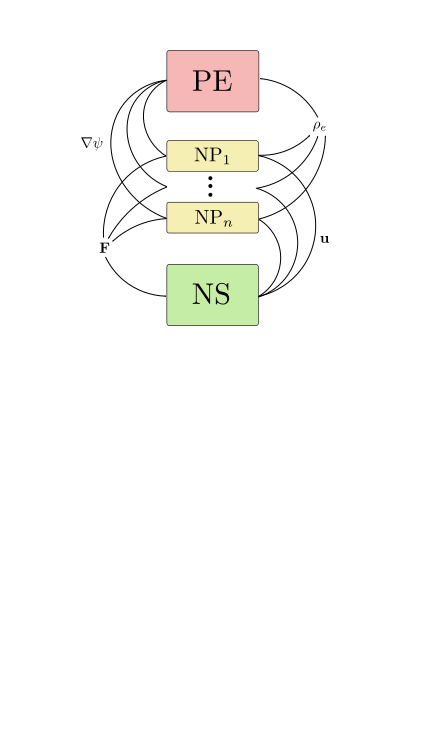
\includegraphics[width=0.5\textwidth]{fig/coupling.pdf}
\end{center}
\caption[Visualisation of the coupling between the equations
  present in the model.]{Visualisation of the coupling between the
  three equations present in the model. Poisson's equation (PE), the
  set of Nernst-Planck equations (NP$_1$ ... NP$_n$) for the different
  ion species and the Navier-Stokes equations (NS). The dependencies
  have also be marked with arrows indicating what quantities for a
  certain equation that are needed from an other.}
\label{fig:coupling}
\end{figure}

%The algorithm to solve the coupled equations is described in section
%\ref{lb:algorithm}.

